\documentclass{article}

\usepackage{upquote} % Upright quotes for verbatim code
\usepackage[mathletters]{ucs} % Extended unicode (utf-8) support
\usepackage{fancyvrb} % verbatim replacement that allows latex
\usepackage{hyperref}
\usepackage{graphicx}
\usepackage{float}

\DefineVerbatimEnvironment{Highlighting}{Verbatim}{commandchars=\\\{\}}
\newcommand{\VerbatimStringTok}[1]{\textcolor[rgb]{0.25,0.44,0.63}{{#1}}}

\graphicspath{ {images/} }

%opening
\title{Algorithms for Big Data - Recommendation System}
\author{Francisco Barros, Francisco Caldeira, Nuno Pires}

\begin{document}

\maketitle

\begin{abstract}
    This project was developed within the scope of Algorithms for Big Data course at ISCTE. 
    In this report we will explain the structure of the dataset used and the approaches that were implemented to create the recommendation system.
\end{abstract}

\section{Introduction}
\label{intro}
In this article we will explain the structure of the dataset used and the approaches that
were implemented to create the recommendation system.
A recommendation system combines several computational techniques to select personalized items based on the
interests of users and conforms to the context in which they are inserted.
Items can be any product, such as movies, books, music, videos, electronic devices, advertisements, etc.
Companies like Google, Youtube, HBO are recognized for their intensive use of recommendation systems.
This kind of systems gives these companies a huge competitive advantage.

Recommendation systems arose in response to people's difficulty in choosing a wide variety of products and services.
These systems have been evolving and nowadays they present a complexity and capacity to make recommendations better
than the human recommendations themselves.

In order to improve the performance of the recommendations, the system approach must be directed to the relationships
between the customers and the items. 
It makes predictions (filtering) about the interests of users and collects the preferences of the various users (collaboration).
For example, if user A has the same opinion as user B about one product then it is more likely that they share
the same opinion in other products than user A sharing the same opinion with a random user.
The similarity between two items is determined by the interest / rating given by the users.

\section{Dataset}
\label{dataset}

For a recommendation system, the dataset must follow some criteria, such as an evaluation system, where it is possible to create a relationship between users and items.
For this project, we chose a dataset collected by Open CDP from an eCommerce store with more than 15 million visitors per month.

TODO

\section{Data Exploration}
\label{data_exploration}

Before implementing the algorithm a data analysis is required to better understand the data at hand.

To start the null values were counted to better evaluate the dataset, the result was:
\begin{Verbatim}[commandchars=\\\{\}]
+--------------+--------+-------------+
|category\_code |brand   |user\_session  |
+--------------+--------+-------------+
|      35413780|15341158|           12|
+--------------+--------+-------------+
\end{Verbatim}
The other columns presented no missing values.


The most purchased and viewed brands were also counted, only showing the top 10.
\begin{Verbatim}[commandchars=\\\{\}]
+--------+------+--------+--------+    
|  Purchased    +     Viewed      |
+--------+------+--------+--------+
|   brand| count|   brand|   count|
+--------+------+--------+--------+
| samsung|372923| samsung|11898628|
|   apple|308937|   apple| 9374247|
|  xiaomi|124908|  xiaomi| 7232401|
|  huawei| 47204|  huawei| 2358235|
|cordiant| 27534| lucente| 1775749|
| lucente| 26137|      lg| 1574848|
|    oppo| 25971|   bosch| 1480771|
|      lg| 21606|    oppo| 1203440|
|    sony| 17038|    sony| 1193071|
|   artel| 15391|    acer| 1084065|
+--------+------+--------+--------+
\end{Verbatim}

The most purchased products with the respective brand and number of purchases
\begin{Verbatim}[commandchars=\\\{\}]
+----------+-------+-----+
|product_id|  brand|count|
+----------+-------+-----+
|   1004856|samsung|61265|
|   1004767|samsung|44419|
|   1005115|  apple|34787|
|   4804056|  apple|30181|
|   1004833|samsung|26183|
|   1002544|  apple|22227|
|   1004870|samsung|21288|
|   1004249|  apple|17971|
|   1005105|  apple|15776|
|   1004836|samsung|15549|
+----------+-------+-----+
\end{Verbatim}
The product id is given since the dataset didn't provide the product commercial name.

%We also plotted the information we deemed useful. The results can be seen below


\section{Data Preparation}
\label{data_prep}

To better handle the algorithm input data some changes had to be done to the dataset,
some columns could be removed and a new one added.

First, three columns were excluded:
\begin{itemize}
    \item \textbf{event\_time} - The event timestamp was removed because it isn't a relevant data for the algorithm used.
    \item \textbf{category\_code} - This column has null values and the dataset already provides a category\_id column with a numeric value to represent the category
    In order not to have redundant information, we decided to exclude it from our dataset.
    \item \textbf{price} - This data is not relevant for our recommendation system, since the algorithm doesn't take the price into consideration.
    The main focus is to establish a relationship between users and products / categories / brands.
\end{itemize}

The new column, named brand\_category, was the concatenation of two others, the category id and brand. This was done to better 
understand the user preference when purchasing items of a given category and their brand of choice.
An example below

\begin{Verbatim}[commandchars=\\\{\}]
    +-------------------+--------+------------------------+
    |category\_id        |brand   |brand\_category           |
    +-------------------+--------+------------------------+
    |2053013552326770905|aqua    |2053013552326770905.aqua|
    +-------------------+--------+------------------------+
\end{Verbatim}

For this project we decided to just consider the events of \textit{view} and \textit{purchase} type since 
in this dataset the \textit{cart} event type doesn't allow to distinguish between the items added to the cart and the removed ones.
Then the dataset was split by event types mencioned above. After to prepare the data for the algorithm several tables were created by grouping the dataset by user\_id and session\_id and
joining the product\_id, category\_id, brand and the new column brand\_category.
This yielded 14 tables that served as an input for the algorithm.
The tables ending with \textit{\_v} represent the views and the others the purchases.
Each table was then saved into a file.
\begin{itemize}
    \item \textbf{user\_products} - user\_id $\times$ product\_id
    \item \textbf{user\_products\_v} - user\_id $\times$ product\_id
    \item \textbf{user\_brands} - user\_id $\times$ brand
    \item \textbf{user\_brands\_v} - user\_id $\times$ brand
    \item \textbf{user\_categories} - user\_id $\times$ category\_id
    \item \textbf{user\_categories\_v} - user\_id $\times$ category\_id
    \item \textbf{user\_category\_brand} - user\_id $\times$ brand\_category
    \item \textbf{user\_category\_brand\_v} - user\_id $\times$ brand\_category
    \item \textbf{session\_products} - session\_id $\times$ brand\_category
    \item \textbf{session\_products\_v} - session\_id $\times$ brand\_category
    \item \textbf{session\_brands }- session\_id $\times$ brand\_category
    \item \textbf{session\_brands\_v} - session\_id $\times$ brand\_category
    \item \textbf{session\_categories} - session\_id $\times$ brand\_category
    \item \textbf{session\_categories\_v} - session\_id $\times$ brand\_category
    \item \textbf{session\_category\_brand} - session\_id $\times$ brand\_category
    \item \textbf{session\_category\_brand\_v} - session\_id $\times$ brand\_category
\end{itemize}

\section{Data analysis}
\label{data-analysis}

Before executing the algorithm, we performed a detailed analysis of the dataset.
Each dataset line is an event specific to an eCommerce store.
Altogether we have 109 950 743 records.
The first step was to identify if there were any null fields.
For this, we built a table with a single line, which shows the field count to null for each column, as shown in the table below.
\begin{center}
    \begin{tabular}{ | c | c | c | } 
        \hline
        \textbf{category\_code} & \textbf{brand} & \textbf{user\_session} \\ 
        \hline
        35 413 780 & 15 341 158 & 12 \\
        \hline
    \end{tabular}
\end{center}
We found many records with \textbf{brand} and \textbf{category\_code} at null and 12 records with \textbf{user\_session} to null.
We decided to remove these lines and not consider them for our recommendation system.
With these changes, we are left with a dataset of 68 650 184 records.

\subsection{Brand analysis}
For the analysis of brands, the quantity of products purchased and viewed from the various brands was counted.
Below are two graphs with this count:

\begin{figure}[H]
    \noindent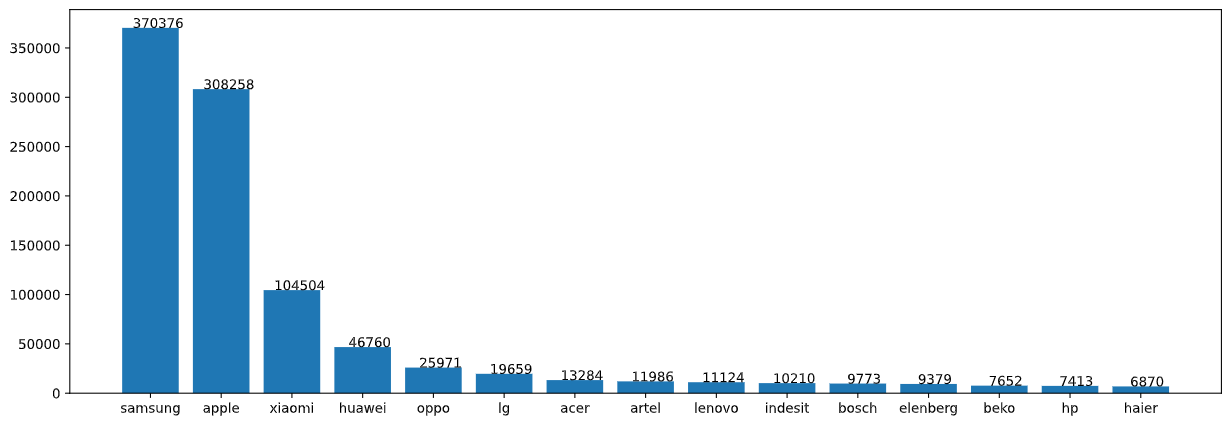
\includegraphics[width=\textwidth]{Count_brand_purchased.png}
    \caption{Count of brand products purchased.}
\end{figure}

\begin{figure}[H]
    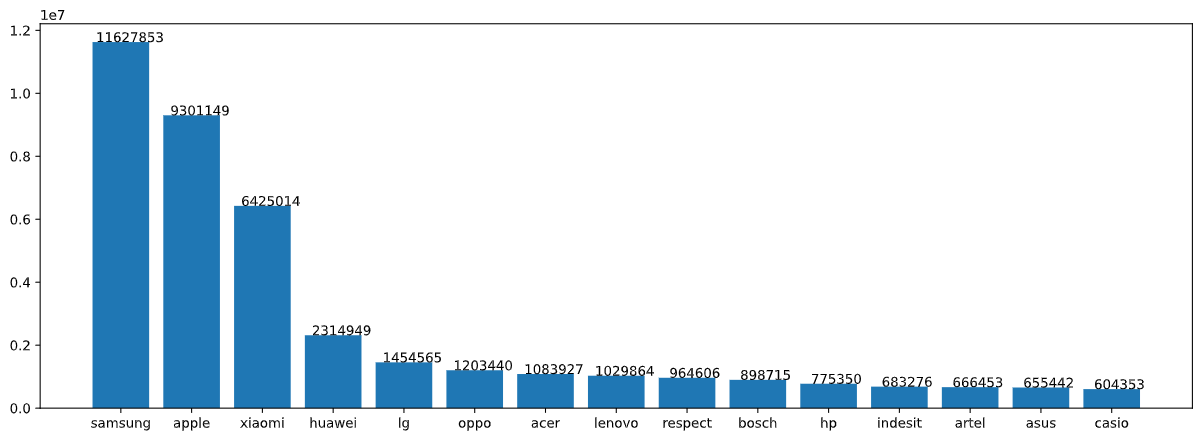
\includegraphics[width=\textwidth]{Count_brand_viewed.png}
    \caption{Count of brand products viewed.}
\end{figure}

As we can see, Samsung was the most viewed and purchased brand.
Apple and Xiaomi are also well represented in this digital store.
An interesting analysis that we can see now is the number of times a brand is seen to be purchased.

\begin{figure}[H]
    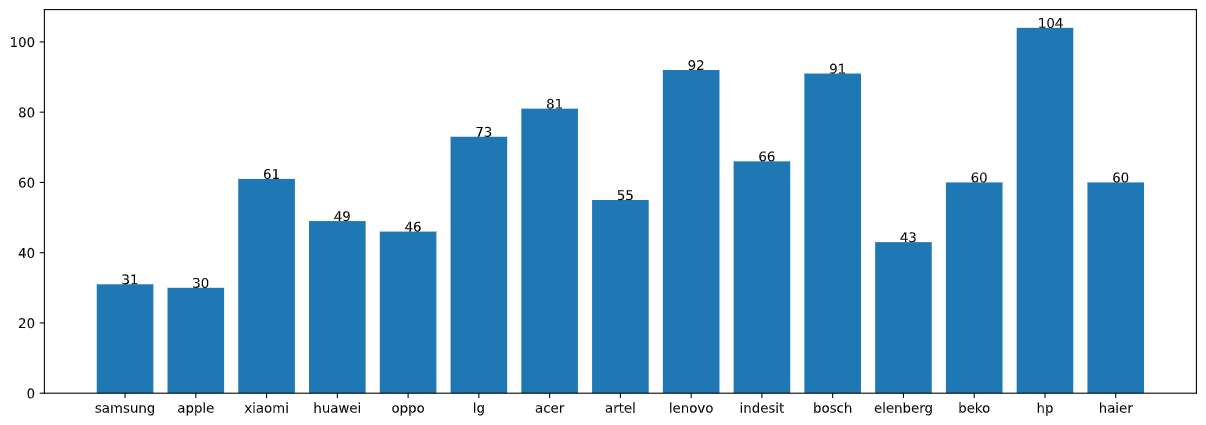
\includegraphics[width=\textwidth]{Brand_viewed_x_purchased.png}
    \caption{Number of times a brand is seen to be purchased.}
\end{figure}

We were able to observe that Samsung and Apple do not need to be seen very often to be purchased.
On the other hand, HP needs to be seen, on average, 104 times before it is purchased.

\subsection{Category analysis}
For the analysis of categories, the number of products by category that were purchased and viewed was analyzed.
Below are two graphs with this count:

\begin{figure}[H]
    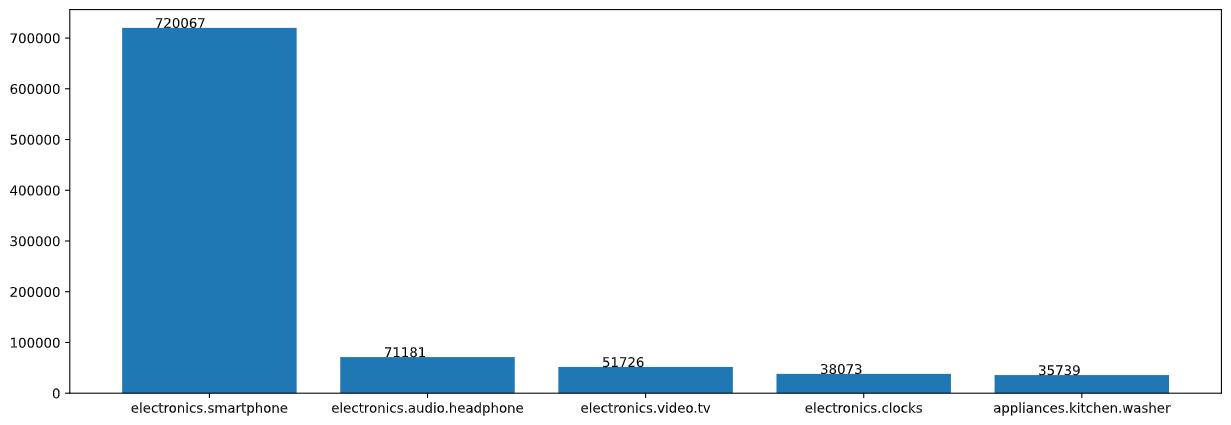
\includegraphics[width=\textwidth]{Count_category_purchased.png}
    \caption{Count of category products purchased.}
\end{figure}

\begin{figure}[H]
    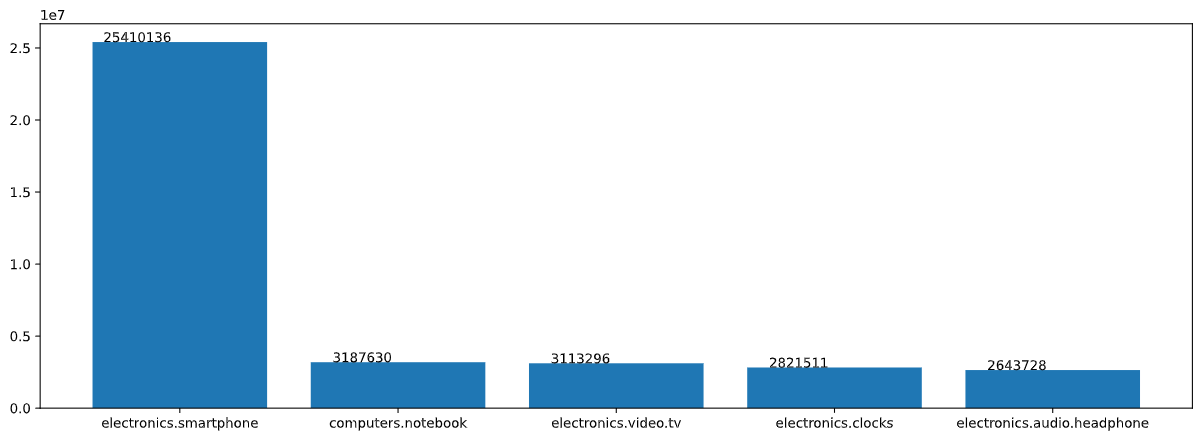
\includegraphics[width=\textwidth]{Count_category_viewed.png}
    \caption{Count of category products viewed.}
\end{figure}

As we can see, smartphones was the most viewed and purchased category, followed by far by computers, TVs, headphones, clocks and kitchen appliances.
An interesting analysis that we can see now is the number of times a category is seen to be purchased.

\begin{figure}[H]
    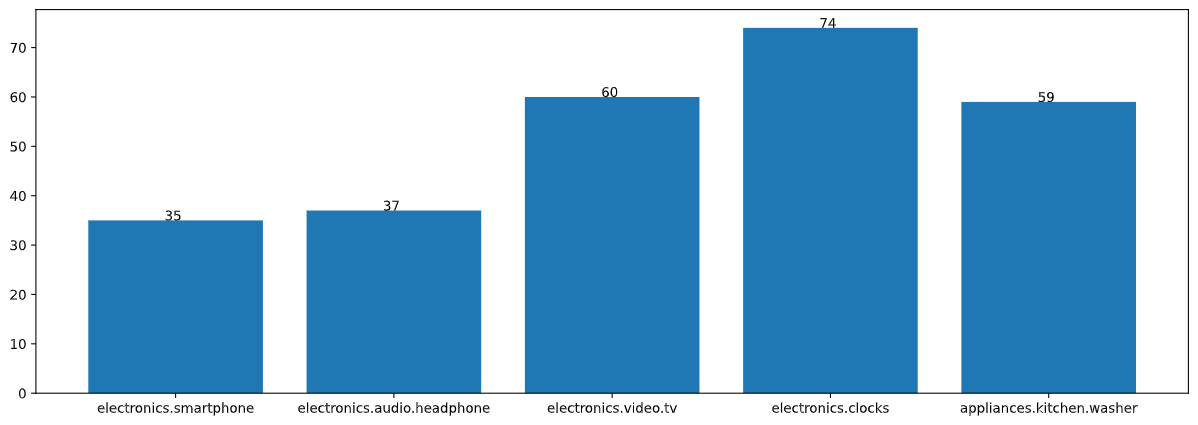
\includegraphics[width=\textwidth]{Category_viewed_x_purchased.png}
    \caption{Number of times a category is seen to be purchased.}
\end{figure}

We were able to observe that smartphones and headphones do not need to be seen very often to be purchased.
On the other hand, clocks needs to be seen, on average, 74 times before it is purchased.


https://towardsdatascience.com/recsys-series-part-4-the-7-variants-of-matrix-factorization-for-collaborative-filtering-368754e4fab5
https://developers.google.com/machine-learning/recommendation/collaborative/matrix

\end{document}


